\chapter{Matrix-Vector Product}

When we take the product of the matrix and the vector, 
it will result in a vector. The product is a contraction 
operation, which means that the matrix's dimension reduced from two to one.
To apply the contraction, then the length of one of the matrix dimensions 
must be the same as the vector's length.

Let the $A$ be the matrix with dimensions $m$ and $n$, 
and the length of the vector $x$ be $n$.

The resultant vector $y$ will have the dimension $m$.

\vspace*{0.5 cm}
$
A = 
\begin{bmatrix}
    a_{00}  & a_{01}    & \dots     & a_{0n}\\
    a_{10}  & a_{11}    & \dots     & a_{1n}\\
    \vdots  & \vdots    & \ddots    & \vdots\\
    a_{m0}  & a_{m1}    & \dots     & a_{mn}\\
\end{bmatrix}
, x =
\begin{bmatrix}
    x_0\\
    x_1\\
    \vdots\\
    x_n\\
\end{bmatrix}
$

\begin{equation}
    y = Ax + y
    \label{eq:mtv}
\end{equation}

$
Av = 
\begin{bmatrix}
    a_{00}  & a_{01}    & \dots     & a_{0n}\\
    a_{10}  & a_{11}    & \dots     & a_{1n}\\
    \vdots  & \vdots    & \ddots    & \vdots\\
    a_{m0}  & a_{m1}    & \dots     & a_{mn}\\
\end{bmatrix}
\begin{bmatrix}
    x_0\\
    x_1\\
    \vdots\\
    x_n\\
\end{bmatrix}
=
\begin{bmatrix}
    \sum_{i=0}^na_{0i}x_i\\
    \sum_{i=0}^na_{1i}x_i\\
    \vdots\\
    \sum_{i=0}^na_{mi}x_i\\
\end{bmatrix}
$

\vspace*{0.5 cm}
The vector times matrix can calculated by taking the transpose on the both sides.
\begin{align*}
    y^T &= (Ax + y)^T\\
    y^T &= (Ax)^T + y^T\\
    y^T &= x^TA^T + y^T\\
\end{align*}

The column-major and row-major layout for the vector in the memory 
is non-distinguishable. Hence, we can use this fact and we get $x = x^T$.
If $A$ is the column-major layout then $A^T$ is the row-major layout and vice-versa.

\begin{equation}
    y = xA^T + y
    \label{eq:vtm}
\end{equation}

\clearpage
\section{Calculating Number of Operations}

Using equation \ref{eq:mtv} or \ref{eq:vtm}, we fill the below table

\begin{table}[ht]
    \centering
    \begin{tabular}{|c|c|}
        \hline
        \textbf{Name} & \textbf{Number} \\
        \hline
        Multiplication & $m$ or $n$\\
        \hline
        Addition & $m-1$ or $n-1$ \\
        \hline
    \end{tabular}
\end{table}

Total Number of Operations $=$ (Number of Multiplication $+$ Number of Addition) $\times
\begin{cases}
    n \\
    m
\end{cases}
$

Total Number of Operations $= 
\begin{cases}
    n \times (m + m - 1)\\
    m  \times (n + n - 1)
\end{cases}
$

Total Number of Operations $= 
\begin{cases}
    n \times (2m - 1)\\
    m  \times (2n - 1)
\end{cases}
$

\section{Algorithm}
The matrix-vector product has two different algorithms: 
Column-Major and Row-Major. We need to handle two different 
layouts differently. 
The Row-Major has the most straightforward algorithm because 
the row elements lay contiguously in the memory, which improves 
the cache locality compared against Column-Major, where the row 
elements placed with a specific stride and hinder the cache locality.

\subsection{Column-Major}

\begin{algorithm}[H]
    \SetAlgoLined
    \SetKwFunction{SIMDFn}{$simd\_loop_N$}
    \SetKwProg{Fn}{Function}{:}{end}

    \tcp{$c$ is the pointer to the output vector}
    \tcp{$a$ is the pointer to the input matrix}
    \tcp{$b$ is the pointer to the input vector}
    \tcp{$block$ is the block of the output vector}
    \tcp{$w$ is the leading dimension of the matrix}
    \tcp{$simd\_loop_N$ is a function where N signifies the amount of the unrolling done}
    \Fn{\SIMDFn($c$, $a$, $b$, $block$, $w$)}{
        \openmp{simd}
        \For{\assign{i}{0} \KwTo $block$ \KwBy $1$}{
            $    
            \begin{matrix}
                c[i] \gets c[i] +  A[i + w * 0] * b[0];\\
                c[i] \gets c[i] +  A[i + w * 1] * b[1];\\
                \vdots\\
                c[i] \gets c[i] +  A[i + w * N] * b[N];\\
            \end{matrix}
            $
        }
    }
    \caption{Matrix-Vector Product SIMD Function}
\end{algorithm}

\begin{algorithm}[H]
    \SetAlgoLined
    \SetKwFunction{SIMDFn}{$main\_loop_N$}
    \SetKwProg{Fn}{Function}{:}{end}

    \tcp{$c$ is the pointer to the output vector}
    \tcp{$a$ is the pointer to the input matrix}
    \tcp{$b$ is the pointer to the input vector}
    \tcp{$n_a$ is the size of the column of the matrix $a$}
    \tcp{$w_a$ is the leading dimension of the matrix $a$}
    \tcp{$n_b$ is the size of the vector $b$}
    \tcp{$block$ is the block of the output vector}
    \tcp{$main\_loop_N$ is a function where N signifies the amount of the unrolling done}
    \Fn{\SIMDFn($c$, $a$, $n_a$, $w_a$, $b$, $n_b$, $block$)}{
        \If{$n_b == 0$}{
            \KwRet{};
        }
        \assignln{ai}{a}
        \assignln{bi}{b}
        \assignln{ci}{c}
        \openmp{for schedule(dynamic)}
        \For{\assign{i}{0} \KwTo $n_a$ \KwBy $block$}{
            \assignln{aj}{ai + i}
            \assignln{bj}{bi}
            \assignln{cj}{ci + i}
            \assignln{ib}{min(block,na-i)}
            \For{\assign{j}{0} \KwTo $n_b$ \KwBy $1$}{
                \assignln{ak}{a + j \times N \times wa}
                \assignln{bk}{bk + j \times N}
                \assignln{ck}{cj}
                $simd\_loop_N(ck,ak,bk,ib,w_a)$
            }
        }
    }
    \caption{Matrix-Vector Product Loop}
\end{algorithm}

\begin{algorithm}[H]
    \SetAlgoLined
    \KwIn{$c$, $a$, $n_a$, $w_a$, $b$, $n_b$, $max\_threads$}
    \tcp{$c$ is the pointer to the output vector}
    \tcp{$a$ and $b$ are pointer to the matrix}
    \tcp{$b$ are pointer to the vector}
    \tcp{$n_a$ is the size of the column of the matrix $a$}
    \tcp{$w_a$ is the leading dimension of the matrix $a$}
    \tcp{$n_b$ is the size of the vector $b$}
    \tcp{$max\_threads$ is the user provided thread count}

    \Begin{
        $omp\_set\_num\_threads(max\_threads)$

        \assignln{number\_el\_L_1}{\lfloor \frac{S_{L_1}}{S_{data}} \rfloor}
        \assignln{half\_block}{\lfloor \frac{number\_el\_L_1}{2} \rfloor}
        \assignln{max\_size}{max(na,nb)}
        \assign{small\_block}{2^{\lfloor \frac{k}{2} \rfloor}}
        \tcp{Where $2^k$ is a power of two representation of $number\_el\_L_1$}
        \assignln{block_2}{max(1, \frac{small\_size}{2^{\lfloor \frac{max\_size}{1024} \rfloor}})}

        \If{$n_a > number\_el\_L_1$}{
            \assignln{block_1}{half\_block}
            }
        \Else{
            \assignln{block_1}{small\_block}
        }

        \assignln{n_{itr}}{\lfloor \frac{n_b}{block_2} \rfloor}
        \assign{n_{rem}}{n_b - (block_2 \times \lfloor \frac{n_b}{block_2} \rfloor)}
        \tcp{This equation gives the remainder}

        \openmp{parallel}
        \Begin{
            $main\_loop_1(c,a,w_a,n_a,b,n_{rem},block_1)$
            
            \assignln{at}{a + w_a \times n_{rem}}
            \assignln{bt}{b + n_{rem}}
            $main\_loop_{block_2}(c,at,w_a,n_a,bt,n_{iter},block_1)$
        }

    }

    \caption{Matrix-Vector Product}
\end{algorithm}

The Column-Major product is quite tricky and complicated if 
we cannot control the instruction set. 
The row elements are $x$ strides away from each other and 
paralyse the cache predictor or cache locality. 
The cache predictor brings the cache line size elements 
from memory, which are place contiguously. 
Each element in the result vector is the product of the 
matrix's row vector and the whole vector. 

For OpenMP to do its magic, we need to fill the $L_1$ cache with 
the result vector block, block of the input vector's matrix and block. 
We divide the load through the threads, where each thread has 
its private cache, and they calculate a small block of the 
result vector without hindering the other vectors. 
The result vector calculation is done by dividing it into 
smaller chunk or block and handing over the block to each thread, 
which removes the dependency within the different blocks and 
eradicates the data races and synchronization. 
The loop which manages the block for the result 
vectors must be multithreaded, and each thread needs to fill 
the $L_1$ cache with the output vector and a column vector of the matrix 
as large as it can so that the registers can fetch the blocks as fast 
as possible from the cache rather than fetching from memory, which adds 
an overhead to the performance. To fit the output vector, the matrix and the vector, 
we previously discussed fact and the \ref{fig:mtv_col_block_diagram} 
for the variable convention; we derive the following equation.

\begin{equation}
    S_{L_1} = S_{data}(m_cn_c + m_c + n_c)
    \label{eq:mtv_col_block} 
\end{equation}

\begin{figure}[htb]
    \centering
    \caption{Matrix-Vector Block Diagram}
    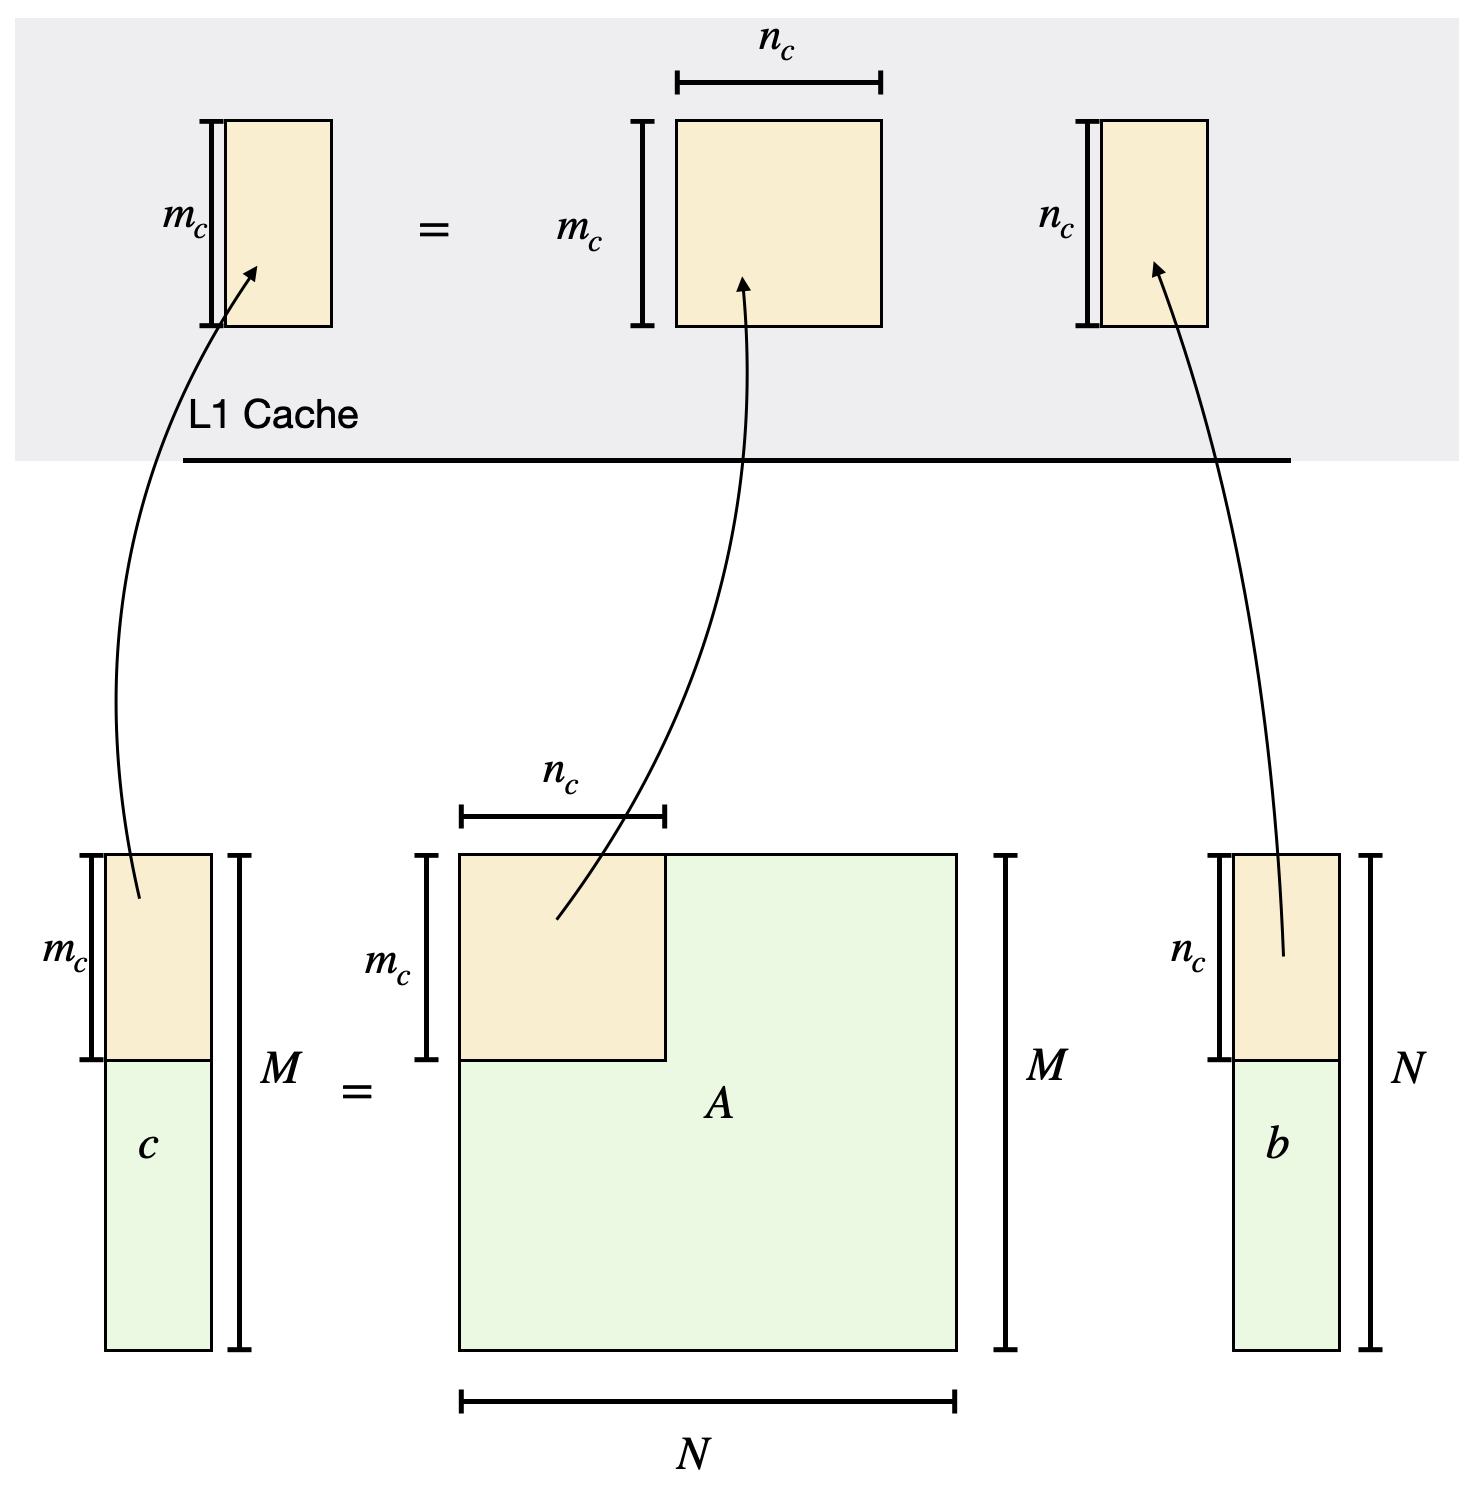
\includegraphics[width=8cm]{../assets/mtv/col_major/block_diagram.png} %
    \label{fig:mtv_col_block_diagram}
\end{figure}


For the small length of the result vector, which is less than the L1 
cache size, to maximize the block in the L1 cache, the row block and 
column block must be identical, $m_c = n_c$, which makes the matrix a square matrix.

Let $m_c = n_c = B_{small}$
\begin{align*}
    S_{L_1} &= S_{data}(m_cn_c + m_c + n_c)\\
    S_{L_1} &= S_{data}(B_{small} \times B_{small} + B_{small} + B_{small})\\
    S_{L_1} &= S_{data}(B_{small}^2 + 2B_{small})\\
\end{align*}

\begin{equation}
    B_{small}^2 + 2B_{small} = \frac{S_{L_1}}{S_{data}}
    \label{eq:mtv_col_small_block} 
\end{equation}

$B_{small}^2$ is much larger than the $2B_{small}$ in \ref{eq:mtv_col_small_block}, so we can ignore the smaller term.

\[B_{small}^2 = \frac{S_{L_1}}{S_{data}}\]

We can represent $\frac{S_{L_1}}{S_{data}}$ in form of power of two because 
we know both $S_{L_1}$ and $S_{data}$ are power of two. Therefore, the division must 
produce a power of two. Let the exponent of two be $k$, which gives us

\[B_{small}^2 = 2^k\]

\begin{equation}
    B_{small} = 2^{\lfloor \frac{k}{2} \rfloor}
    \label{eq:mtv_col_small_block_simplified} 
\end{equation}

The eqauation \ref{eq:mtv_col_small_block_simplified} is only valid if the length of the output
vector is less than the $L_1$ cache.

\clearpage
\subsection{Row-Major}

\begin{algorithm}[H]
    \SetAlgoLined
    \SetKwFunction{SIMDFn}{$simd\_loop$}
    \SetKwProg{Fn}{Function}{:}{end}

    \tcp{$a$ is the pointer to the input matrix}
    \tcp{$b$ is the pointer to the input vector}
    \tcp{$n_b$ is the block of the output vector}
    \Fn{\SIMDFn($a$, $b$, $n_b$)}{
        \assignln{sum}{0}
        \openmp{simd}
        \For{\assign{i}{0} \KwTo $n_b$ \KwBy $1$}{
            \assignln{sum}{sum + a[i] \times b[i]}
        }
        \KwRet{sum}
    }
    \caption{Matrix-Vector Product SIMD Function}
\end{algorithm}

\begin{algorithm}[H]
    \SetAlgoLined
    \KwIn{$c$, $a$, $n_a$, $w_a$, $b$, $n_b$, $max\_threads$}
    \tcp{$c$ is the pointer to the output vector}
    \tcp{$a$ and $b$ are pointer to the matrix}
    \tcp{$b$ are pointer to the vector}
    \tcp{$n_a$ is the size of the column of the matrix $a$}
    \tcp{$w_a$ is the leading dimension of the matrix $a$}
    \tcp{$n_b$ is the size of the vector $b$}
    \tcp{$max\_threads$ is the user provided thread count}

    \Begin{
        $omp\_set\_num\_threads(max\_threads)$

        \assignln{ai}{a}
        \assignln{bi}{b}
        \assignln{ci}{c}
        
        \openmp{parallel for schedule(static)}
        \For{\assign{i}{0} \KwTo $n_a$ \KwBy $1$}{
            \assignln{aj}{ai + i * w_a}
            \assignln{bj}{bi}
            \assignln{cj}{ci + i}
            \assignln{cj}{simd\_loop(aj,bj,n_b)}
        }
    }

    \caption{Matrix-Vector Product}
\end{algorithm}

\clearpage
\section{Performance Plots and Speedup Summary For Column-Major}

\begin{figure}[htb]
    \centering
    \caption*{Performance measurements of ?gemv implementations}
    \subfloat[\centering Single-Precision]{{\includegraphics[width=8cm]{../assets/mtv/col_major/float_GflopsVsSize.png} }}%
    \label{fig:mtv_col_Sgflop220}
    \qquad
    \subfloat[\centering Double-Precision]{{\includegraphics[width=8cm]{../assets/mtv/col_major/double_GflopsVsSize.png} }}%
    \label{fig:mtv_col_Dgflop220}
\end{figure}

\begin{figure}[htb]
    \centering
    \caption*{Sorted performance measurements of ?gemv implementations}
    \subfloat[\centering Single-Precision]{{\includegraphics[width=8cm]{../assets/mtv/col_major/float_GflopsVsSize_per.png} }}%
    \label{fig:mtv_col_Sgflop_per220}
    \qquad
    \subfloat[\centering Double-Precision]{{\includegraphics[width=8cm]{../assets/mtv/col_major/double_GflopsVsSize_per.png} }}%
    \label{fig:mtv_col_Dgflop_per220}
\end{figure}

\begin{figure}[htb]
    \centering
    \caption*{Comparison of the Boost.uBLAS.Tensor ?gemv implementation}
    \subfloat[\centering Single-Precision]{{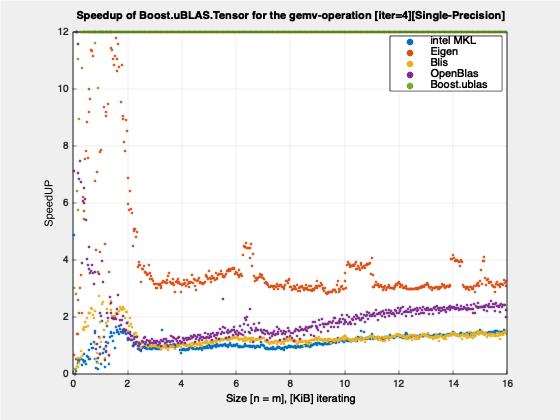
\includegraphics[width=8cm]{../assets/mtv/col_major/float_Speedup.png} }}%
    \label{fig:mtv_col_Sspeedup220}
    \qquad
    \subfloat[\centering Double-Precision]{{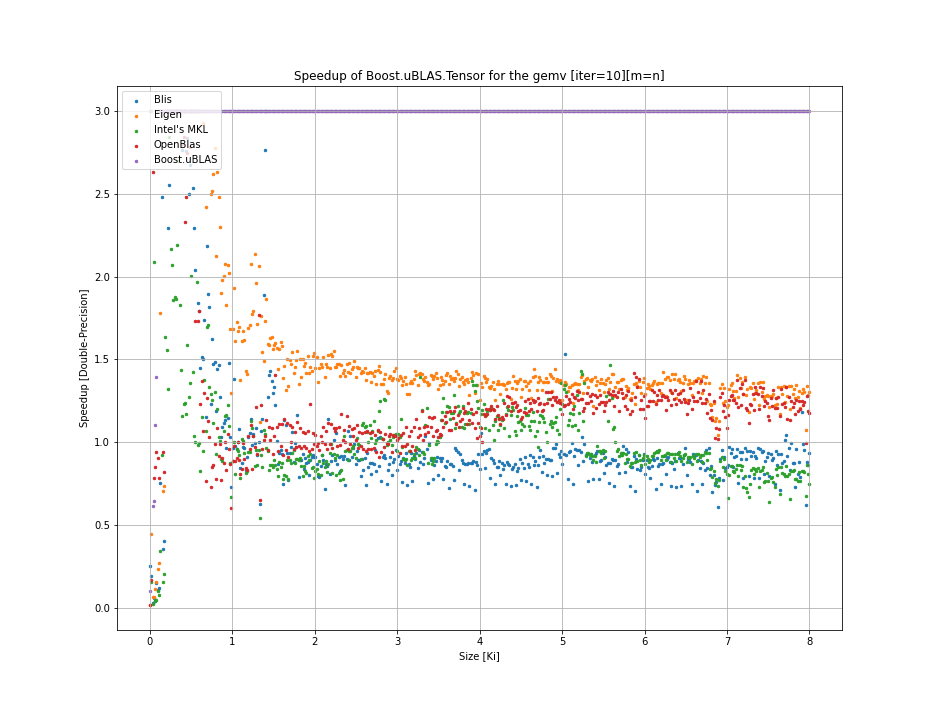
\includegraphics[width=8cm]{../assets/mtv/col_major/double_Speedup.png} }}%
    \label{fig:mtv_col_Dspeedup220}
\end{figure}

\begin{figure}[htb]
    \centering
    \caption*{Comparison of the Boost.uBLAS.Tensor ?gemv implementation [semilogy]}
    \subfloat[\centering Single-Precision]{{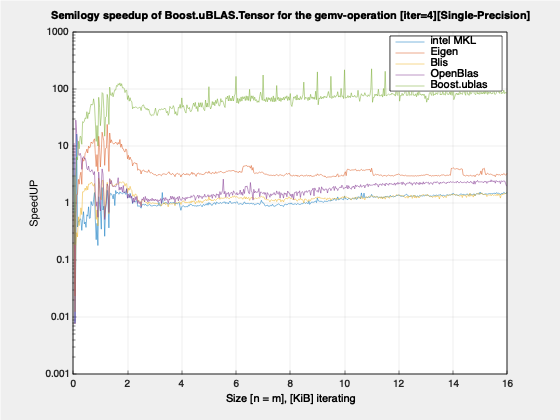
\includegraphics[width=8cm]{../assets/mtv/col_major/float_Speedup_log10.png} }}%
    \label{fig:mtv_col_Sspeedup_log10220}
    \qquad
    \subfloat[\centering Double-Precision]{{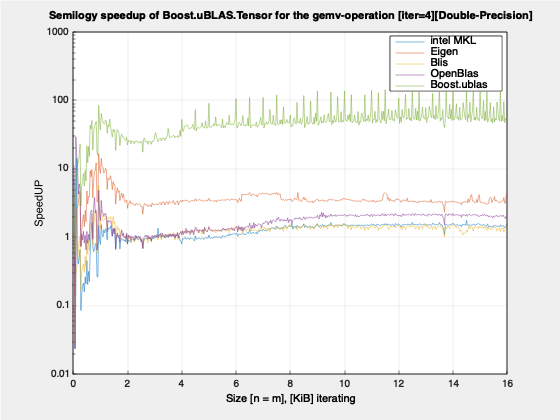
\includegraphics[width=8cm]{../assets/mtv/col_major/double_Speedup_log10.png} }}%
    \label{fig:mtv_col_Dspeedup_log10220}
\end{figure}

\begin{figure}[htb]
    \centering
    \caption*{Comparison of the Boost.uBLAS.Tensor ?gemv implementation [sorted]}
    \subfloat[\centering Single-Precision]{{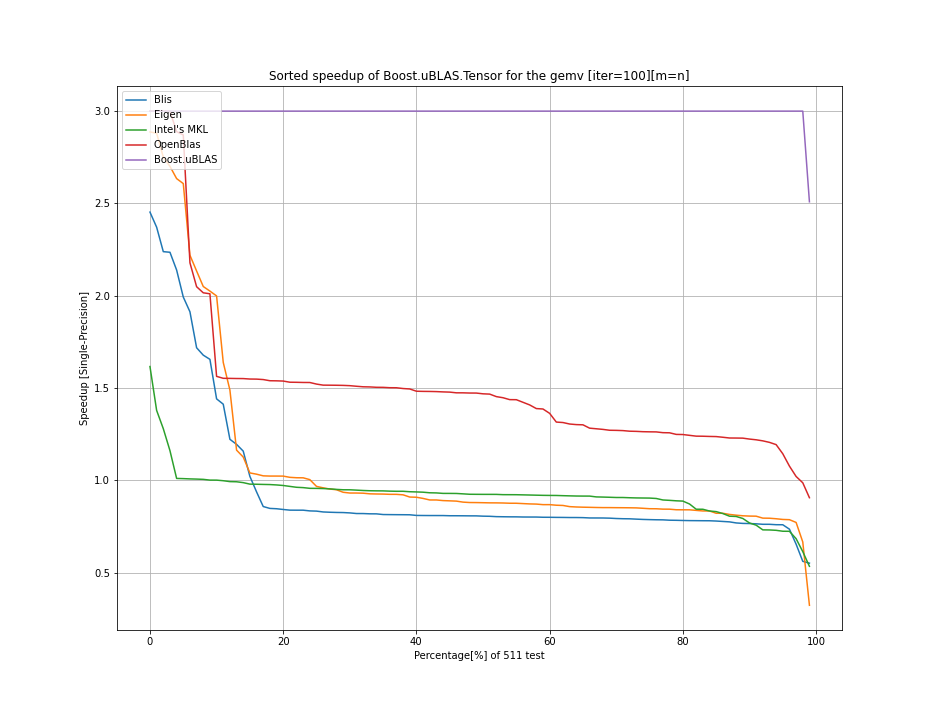
\includegraphics[width=8cm]{../assets/mtv/col_major/float_Speedup_per.png} }}%
    \label{fig:mtv_col_Sspeedup_per220}
    \qquad
    \subfloat[\centering Double-Precision]{{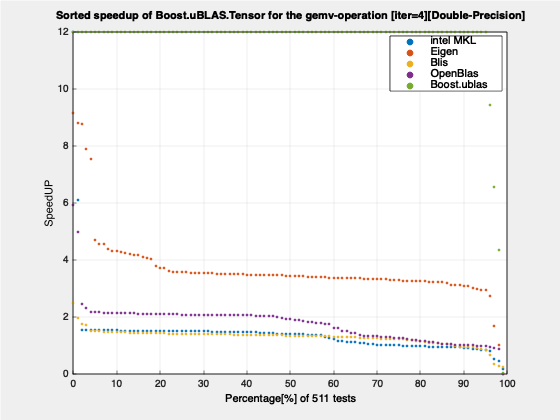
\includegraphics[width=8cm]{../assets/mtv/col_major/double_Speedup_per.png} }}%
    \label{fig:mtv_col_Dspeedup_per220}
\end{figure}

\begin{table}[ht]
    \centering
    \caption{Speedup Summary For Single-Precision}
    \begin{tabular}{|l|c|c|}
        \hline
        \textbf{Implementation} & \textbf{Speedup $\geq$ 1 [\%]} & \textbf{Speedup $\geq$ 2 [\%]}\\
        \hline
        Boost.uBLAS & $97$ & $97$ \\
        \hline
        OpenBLAS    & $98$ & $8$ \\
        \hline
        Eigen       & $97$ & $96$ \\
        \hline
        Blis        & $65$ & $5$ \\
        \hline
        Intel's MKL & $52$ & $1$ \\
        \hline
    \end{tabular}
    
    \begin{tabular}{|l|c|c|}
        \hline
        \textbf{Implementation} & \textbf{Speed-down $\geq$ 1 [\%]} & \textbf{Speed-down $\geq$ 2 [\%]}\\
        \hline
        Boost.uBLAS & $1$ & $1$ \\
        \hline
        OpenBLAS    & $0$ & $0$ \\
        \hline
        Eigen       & $1$ & $1$ \\
        \hline
        Blis        & $33$ & $1$ \\
        \hline
        Intel's MKL & $46$ & $1$ \\
        \hline
    \end{tabular}
    
    \vspace*{1 cm}

    \centering
    \caption{Speedup Summary For Double-Precision}
    \begin{tabular}{|l|c|c|}
        \hline
        \textbf{Implementation} & \textbf{Speedup $\geq$ 1 [\%]} & \textbf{Speedup $\geq$ 2 [\%]}\\
        \hline
        Boost.uBLAS & $98$ & $97$ \\
        \hline
        OpenBLAS    & $87$ & $31$ \\
        \hline
        Eigen       & $98$ & $97$ \\
        \hline
        Blis        & $82$ & $0$ \\
        \hline
        Intel's MKL & $75$ & $2$ \\
        \hline
    \end{tabular}
    
    \begin{tabular}{|l|c|c|}
        \hline
        \textbf{Implementation} & \textbf{Speed-down $\geq$ 1 [\%]} & \textbf{Speed-down $\geq$ 2 [\%]}\\
        \hline
        Boost.uBLAS & $0$ & $0$ \\
        \hline
        OpenBLAS    & $11$ & $0$ \\
        \hline
        Eigen       & $0$ & $0$ \\
        \hline
        Blis        & $16$ & $1$ \\
        \hline
        Intel's MKL & $23$ & $0$ \\
        \hline
    \end{tabular}
\end{table}

\clearpage
\section{Performance Metrics For Column-Major}

\subsection*{Range[Start: $32$, End: $16382$, Step: $32$]}

\begin{table}[ht]
    \centering
    \caption{GFLOPS For Single-Precision}
    \begin{tabular}{|l|c|c|}
        \hline
        \textbf{Implementation} & \textbf{Max} & \textbf{Average}\\
        \hline
        Boost.uBLAS.Tensor  & $68.657$& $15.4648$ \\
        \hline
        Boost.uBLAS         & $1.88885$& $0.36405$ \\
        \hline
        Intel's MKL         & $82.9976$& $16.2728$ \\
        \hline
        OpenBLAS            & $31.0462$& $9.46484$ \\
        \hline
        Blis                & $28.7954$& $12.5415$ \\
        \hline
        Eigen               & $11.2304$& $3.85244$ \\
        \hline
    \end{tabular}

    \vspace*{1 cm}

    \centering
    \caption{GFLOPS For Double-Precision}
    \begin{tabular}{|l|c|c|}
        \hline
        \textbf{Implementation} & \textbf{Max} & \textbf{Average}\\
        \hline
        Boost.uBLAS.Tensor  & $35.6327$ & $7.39512$ \\
        \hline
        Boost.uBLAS         & $1.19679$ & $0.254521$ \\
        \hline
        Intel's MKL         & $34.9999$ & $6.91274$ \\
        \hline
        OpenBLAS            & $12.4044$ & $4.59443$ \\
        \hline
        Blis                & $14.1552$ & $5.86746$ \\
        \hline
        Eigen               & $4.72151$ & $2.07815$ \\
        \hline
    \end{tabular}
\end{table}

\begin{table}[ht]
    \centering
    \caption{Utilization[\%] For Single-Precision}
    \begin{tabular}{|l|c|c|}
        \hline
        \textbf{Implementation} & \textbf{Max} & \textbf{Average}\\
        \hline
        Boost.uBLAS.Tensor  & $11.6605$& $2.62649$ \\
        \hline
        Boost.uBLAS         & $0.320797$& $0.0618291$ \\
        \hline
        Intel's MKL         & $14.0961$& $2.76373$ \\
        \hline
        OpenBLAS            & $5.2728$& $1.60748$ \\
        \hline
        Blis                & $4.89052$& $2.13$ \\
        \hline
        Eigen               & $1.90734$& $0.654287$ \\
        \hline
    \end{tabular}

    \vspace*{1 cm}

    \centering
    \caption{Utilization[\%] For Double-Precision}
    \begin{tabular}{|l|c|c|}
        \hline
        \textbf{Implementation} & \textbf{Max} & \textbf{Average}\\
        \hline
        Boost.uBLAS.Tensor  & $12.1035$ & $2.51193$ \\
        \hline
        Boost.uBLAS         & $0.406518$ & $0.0864542$ \\
        \hline
        Intel's MKL         & $11.8886$ & $2.34808$ \\
        \hline
        OpenBLAS            & $4.21346$ & $1.56061$ \\
        \hline
        Blis                & $4.80814$ & $1.99302$ \\
        \hline
        Eigen               & $1.60378$ & $0.705893$ \\
        \hline
    \end{tabular}
\end{table}

\begin{table}[ht]
    \centering
    \caption{Speedup(Boost.uBLAS.Tensor) For Single-Precision}
    \begin{tabular}{|l|c|c|}
        \hline
        \textbf{Implementation} & \textbf{Max} & \textbf{Average}\\
        \hline
        Boost.uBLAS         & $36.3486$ & $42.4797$ \\
        \hline
        Intel's MKL         & $0.827217$ & $0.950343$ \\
        \hline
        OpenBLAS            & $2.21144$ & $1.63392$ \\
        \hline
        Blis                & $2.38431$ & $1.23309$ \\
        \hline
        Eigen               & $6.1135$ & $4.01427$ \\
        \hline
    \end{tabular}

    \vspace*{1 cm}

    \centering
    \caption{Speedup(Boost.uBLAS.Tensor) For Double-Precision}
    \begin{tabular}{|l|c|c|}
        \hline
        \textbf{Implementation} & \textbf{Max} & \textbf{Average}\\
        \hline
        Boost.uBLAS         & $29.7735$ & $29.055$ \\
        \hline
        Intel's MKL         & $1.01808$ & $1.06978$ \\
        \hline
        OpenBLAS            & $2.87258$ & $1.60958$ \\
        \hline
        Blis                & $2.51729$ & $1.26036$ \\
        \hline
        Eigen               & $7.54688$ & $3.55852$ \\
        \hline
    \end{tabular}
\end{table}

\clearpage
\section{Performance Plots and Speedup Summary For Row-Major}

\begin{figure}[htb]
    \centering
    \caption*{Performance measurements of ?gemv implementations}
    \subfloat[\centering Single-Precision]{{\includegraphics[width=8cm]{../assets/mtv/row_major/float_GflopsVsSize.png} }}%
    \label{fig:mtv_row_Sgflop220}
    \qquad
    \subfloat[\centering Double-Precision]{{\includegraphics[width=8cm]{../assets/mtv/row_major/double_GflopsVsSize.png} }}%
    \label{fig:mtv_row_Dgflop220}
\end{figure}

\begin{figure}[htb]
    \centering
    \caption*{Sorted performance measurements of ?gemv implementations}
    \subfloat[\centering Single-Precision]{{\includegraphics[width=8cm]{../assets/mtv/row_major/float_GflopsVsSize_per.png} }}%
    \label{fig:mtv_row_Sgflop_per220}
    \qquad
    \subfloat[\centering Double-Precision]{{\includegraphics[width=8cm]{../assets/mtv/row_major/double_GflopsVsSize_per.png} }}%
    \label{fig:mtv_row_Dgflop_per220}
\end{figure}

\begin{figure}[htb]
    \centering
    \caption*{Comparison of the Boost.uBLAS.Tensor ?gemv implementation}
    \subfloat[\centering Single-Precision]{{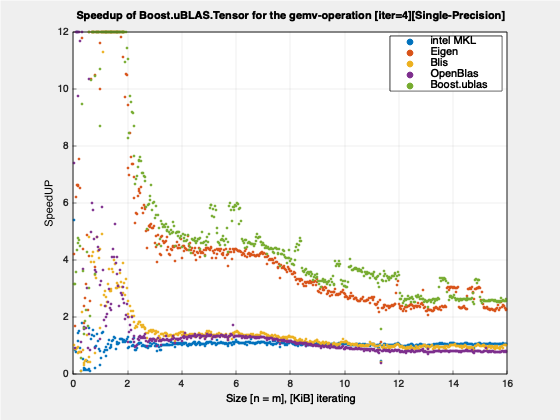
\includegraphics[width=8cm]{../assets/mtv/row_major/float_Speedup.png} }}%
    \label{fig:mtv_row_Sspeedup220}
    \qquad
    \subfloat[\centering Double-Precision]{{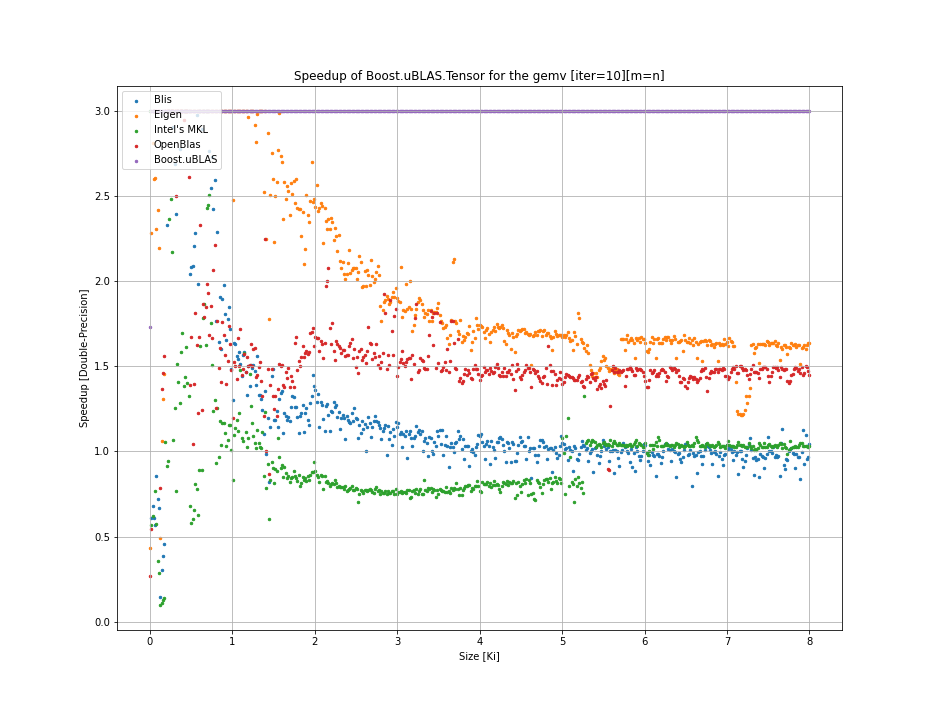
\includegraphics[width=8cm]{../assets/mtv/row_major/double_Speedup.png} }}%
    \label{fig:mtv_row_Dspeedup220}
\end{figure}

\begin{figure}[htb]
    \centering
    \caption*{Comparison of the Boost.uBLAS.Tensor ?gemv implementation [semilogy]}
    \subfloat[\centering Single-Precision]{{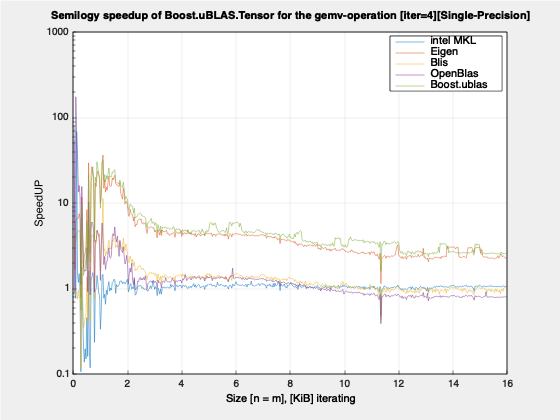
\includegraphics[width=8cm]{../assets/mtv/row_major/float_Speedup_log10.png} }}%
    \label{fig:mtv_row_Sspeedup_log10220}
    \qquad
    \subfloat[\centering Double-Precision]{{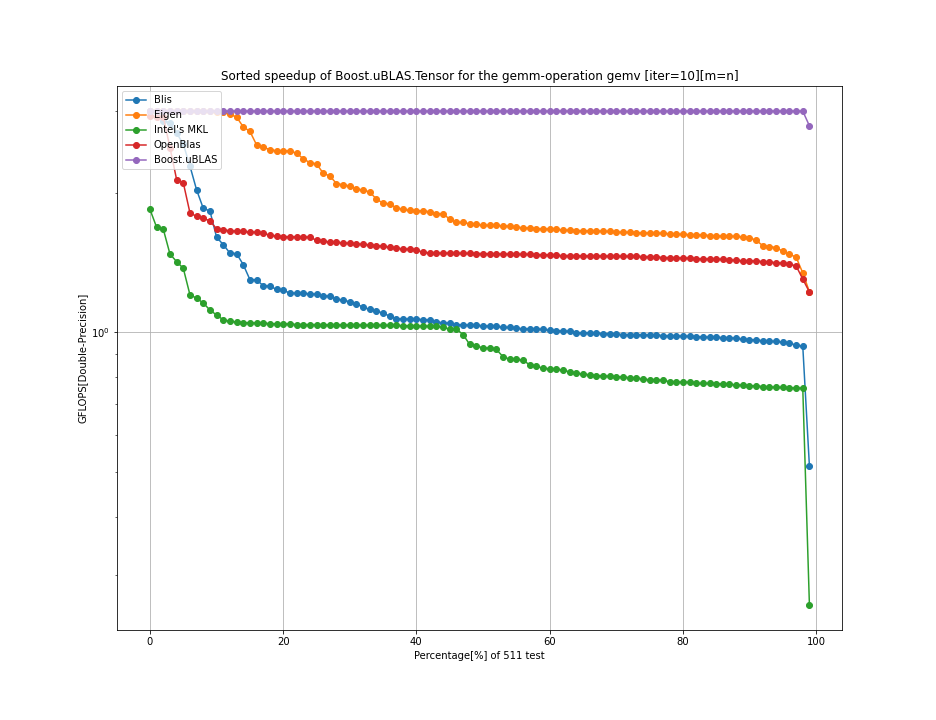
\includegraphics[width=8cm]{../assets/mtv/row_major/double_Speedup_log10.png} }}%
    \label{fig:mtv_row_Dspeedup_log10220}
\end{figure}

\begin{figure}[htb]
    \centering
    \caption*{Comparison of the Boost.uBLAS.Tensor ?gemv implementation [sorted]}
    \subfloat[\centering Single-Precision]{{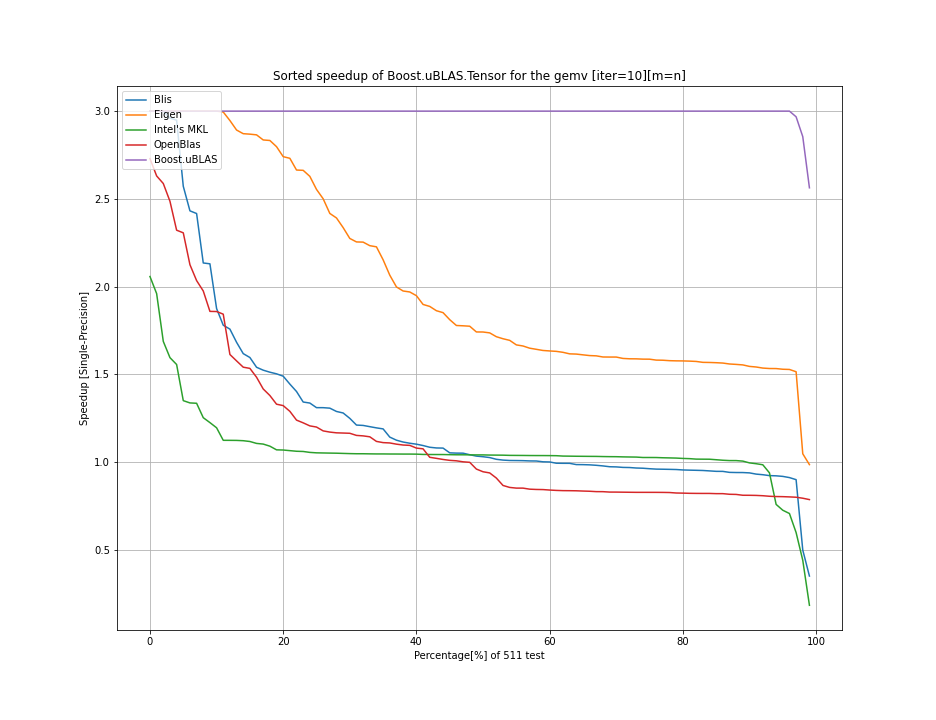
\includegraphics[width=8cm]{../assets/mtv/row_major/float_Speedup_per.png} }}%
    \label{fig:mtv_row_Sspeedup_per220}
    \qquad
    \subfloat[\centering Double-Precision]{{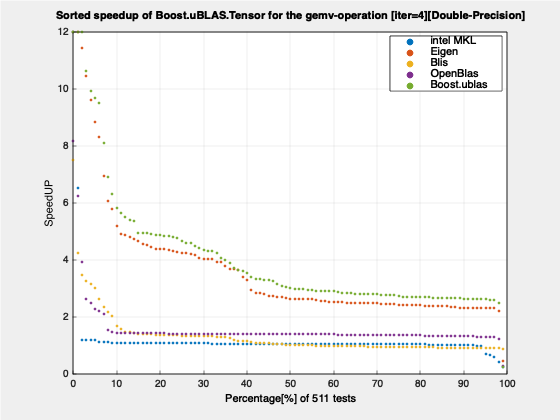
\includegraphics[width=8cm]{../assets/mtv/row_major/double_Speedup_per.png} }}%
    \label{fig:mtv_row_Dspeedup_per220}
\end{figure}

\begin{table}[ht]
    \centering
    \caption{Speedup Summary For Single-Precision}
    \begin{tabular}{|l|c|c|}
        \hline
        \textbf{Implementation} & \textbf{Speedup $\geq$ 1 [\%]} & \textbf{Speedup $\geq$ 2 [\%]}\\
        \hline
        Boost.uBLAS & $98$ & $98$ \\
        \hline
        OpenBLAS    & $56$ & $10$ \\
        \hline
        Eigen       & $98$ & $97$ \\
        \hline
        Blis        & $73$ & $9$ \\
        \hline
        Intel's MKL & $88$ & $1$ \\
        \hline
    \end{tabular}
    
    \begin{tabular}{|l|c|c|}
        \hline
        \textbf{Implementation} & \textbf{Speed-down $\geq$ 1 [\%]} & \textbf{Speed-down $\geq$ 2 [\%]}\\
        \hline
        Boost.uBLAS & $0$ & $0$ \\
        \hline
        OpenBLAS    & $42$ & $0$ \\
        \hline
        Eigen       & $0$ & $0$ \\
        \hline
        Blis        & $25$ & $0$ \\
        \hline
        Intel's MKL & $10$ & $0$ \\
        \hline
    \end{tabular}
    
    \vspace*{1 cm}

    \centering
    \caption{Speedup Summary For Double-Precision}
    \begin{tabular}{|l|c|c|}
        \hline
        \textbf{Implementation} & \textbf{Speedup $\geq$ 1 [\%]} & \textbf{Speedup $\geq$ 2 [\%]}\\
        \hline
        Boost.uBLAS & $98$ & $98$ \\
        \hline
        OpenBLAS    & $98$ & $7$ \\
        \hline
        Eigen       & $98$ & $98$ \\
        \hline
        Blis        & $59$ & $9$ \\
        \hline
        Intel's MKL & $92$ & $1$ \\
        \hline
    \end{tabular}
    
    \begin{tabular}{|l|c|c|}
        \hline
        \textbf{Implementation} & \textbf{Speed-down $\geq$ 1 [\%]} & \textbf{Speed-down $\geq$ 2 [\%]}\\
        \hline
        Boost.uBLAS & $0$ & $0$ \\
        \hline
        OpenBLAS    & $0$ & $0$ \\
        \hline
        Eigen       & $0$ & $0$ \\
        \hline
        Blis        & $39$ & $0$ \\
        \hline
        Intel's MKL & $6$ & $1$ \\
        \hline
    \end{tabular}
\end{table}

\clearpage
\section{Performance Metrics For Row-Major}

\subsection*{Range[Start: $32$, End: $16382$, Step: $32$]}

\begin{table}[ht]
    \centering
    \caption{GFLOPS For Single-Precision}
    \begin{tabular}{|l|c|c|}
        \hline
        \textbf{Implementation} & \textbf{Max} & \textbf{Average}\\
        \hline
        Boost.uBLAS.Tensor  & $114.495$& $19.4496$ \\
        \hline
        Boost.uBLAS         & $4.86818$& $3.62716$ \\
        \hline
        Intel's MKL         & $103.86$& $19.2955$ \\
        \hline
        OpenBLAS            & $39.0813$& $14.0183$ \\
        \hline
        Blis                & $28.5224$& $12.8971$ \\
        \hline
        Eigen               & $8.70003$& $4.11144$ \\
        \hline
    \end{tabular}

    \vspace*{1 cm}

    \centering
    \caption{GFLOPS For Double-Precision}
    \begin{tabular}{|l|c|c|}
        \hline
        \textbf{Implementation} & \textbf{Max} & \textbf{Average}\\
        \hline
        Boost.uBLAS.Tensor  & $48.6174$& $8.13646$ \\
        \hline
        Boost.uBLAS         & $2.19048$& $1.82291$ \\
        \hline
        Intel's MKL         & $51.6863$& $8.51818$ \\
        \hline
        OpenBLAS            & $18.6354$& $5.19158$ \\
        \hline
        Blis                & $14.9491$& $6.06728$ \\
        \hline
        Eigen               & $6.28753$& $2.04718$ \\
        \hline
    \end{tabular}
\end{table}

\begin{table}[ht]
    \centering
    \caption{Utilization[\%] For Single-Precision}
    \begin{tabular}{|l|c|c|}
        \hline
        \textbf{Implementation} & \textbf{Max} & \textbf{Average}\\
        \hline
        Boost.uBLAS.Tensor  & $19.4456$& $3.30327$ \\
        \hline
        Boost.uBLAS         & $0.826797$& $0.616026$ \\
        \hline
        Intel's MKL         & $17.6393$& $3.27708$ \\
        \hline
        OpenBLAS            & $6.63744$& $2.38082$ \\
        \hline
        Blis                & $4.84416$& $2.1904$ \\
        \hline
        Eigen               & $1.47759$& $0.698275$ \\
        \hline
    \end{tabular}

    \vspace*{1 cm}

    \centering
    \caption{Utilization[\%] For Double-Precision}
    \begin{tabular}{|l|c|c|}
        \hline
        \textbf{Implementation} & \textbf{Max} & \textbf{Average}\\
        \hline
        Boost.uBLAS.Tensor  & $16.5141$& $2.76374$ \\
        \hline
        Boost.uBLAS         & $0.744048$& $0.619195$ \\
        \hline
        Intel's MKL         & $17.5565$& $2.89341$ \\
        \hline
        OpenBLAS            & $6.32996$& $1.76344$ \\
        \hline
        Blis                & $5.07782$& $2.0609$ \\
        \hline
        Eigen               & $2.13571$& $0.695374$ \\
        \hline
    \end{tabular}
\end{table}

\begin{table}[ht]
    \centering
    \caption{Speedup(Boost.uBLAS.Tensor) For Single-Precision}
    \begin{tabular}{|l|c|c|}
        \hline
        \textbf{Implementation} & \textbf{Max} & \textbf{Average}\\
        \hline
        Boost.uBLAS         & $23.5192$& $5.36222$ \\
        \hline
        Intel's MKL         & $1.1024$& $1.00799$ \\
        \hline
        OpenBLAS            & $2.92968$& $1.38745$ \\
        \hline
        Blis                & $4.01423$& $1.50807$ \\
        \hline
        Eigen               & $13.1604$& $4.73061$ \\
        \hline
    \end{tabular}

    \vspace*{1 cm}

    \centering
    \caption{Speedup(Boost.uBLAS.Tensor) For Double-Precision}
    \begin{tabular}{|l|c|c|}
        \hline
        \textbf{Implementation} & \textbf{Max} & \textbf{Average}\\
        \hline
        Boost.uBLAS         & $22.1949$& $4.46344$ \\
        \hline
        Intel's MKL         & $0.940624$& $0.955187$ \\
        \hline
        OpenBLAS            & $2.60887$& $1.56724$ \\
        \hline
        Blis                & $3.25219$& $1.34104$ \\
        \hline
        Eigen               & $7.73235$& $3.97447$ \\
        \hline
    \end{tabular}
\end{table}